%%%%%%%%%%%%%%%%%%%%%%%%%%%%%%%%%%%%%%%%
\subsection{Data Preprocessing}
The LI-EKF is tested with two types of data, i.e., simulated data generated by the group and Zurich Urban Micro Aerial Vehicle Dataset \cite{majdik2017zurich}. 

Onboard Pose data from PX4 autopilot board and onboard GPS data are utilized. GPS data is in international WGS 84 (GPS) coordinate system, which are transformed into world frame and aligned with pose coordination system. The noise covariance matrix of the GPS is calculated by taking the covariant of error between GPS and the ground truth data included in the Dataset. 

%%%%%%%%%%%%%%%%%%%%%%%%%%%%%%%%%%%%%%%%
\subsection{Verification with Simulated Data}

We ran a series of tests using a generated set of data to test the accuracy of the filter and test its robustness to input noise.  The set of tests was run on the MATLAB version of the filter in order to use the built in plotting feature to provide a visual verification.  We also used the simulated data tests to generate test cases for the C++ version of the filter, which are added as additional tests in its testing suite.

The simulated data consists of a set of state variables and their derivatives, created from a set of random polynomials which are functions of time.  First, we generate six polynomials, three for the position $(x, y, z)$ in the world frame and three for the angle axis rotation of the body frame with respect to the world frame.  From the position polynomials, we take the derivative once to get the velocity as a function of time and once more to get the acceleration.  Using the time data input as a parameter, we sample the polynomials at the desired time points and save the data.  We similarly generate rotation matrices from the angle axis polynomials for each time point, and take the discrete derivative between time points to find the angular rates.  The world frame acceleration is then rotated into the body frame, after having the gravity bias that an accelerometer would measure added to it.  At the end of the procedure, we provide ourselves with simulated IMU measurements along with the exact ground truth data from which it was generated.

While simulation on "perfect" simulated data can be a good first check for the filter, we also verify the filter after corrupting the simulated data with random noise.  In order to more closely simulate the measurements obtained by a real IMU, we add zero mean Gaussian noise to the angular rate and body frame acceleration measurements. The noise has a tunable covariance parameter to achieve the desired noise level.

% polynomials seeded with rng(2)
\begin{figure}
    \centering
    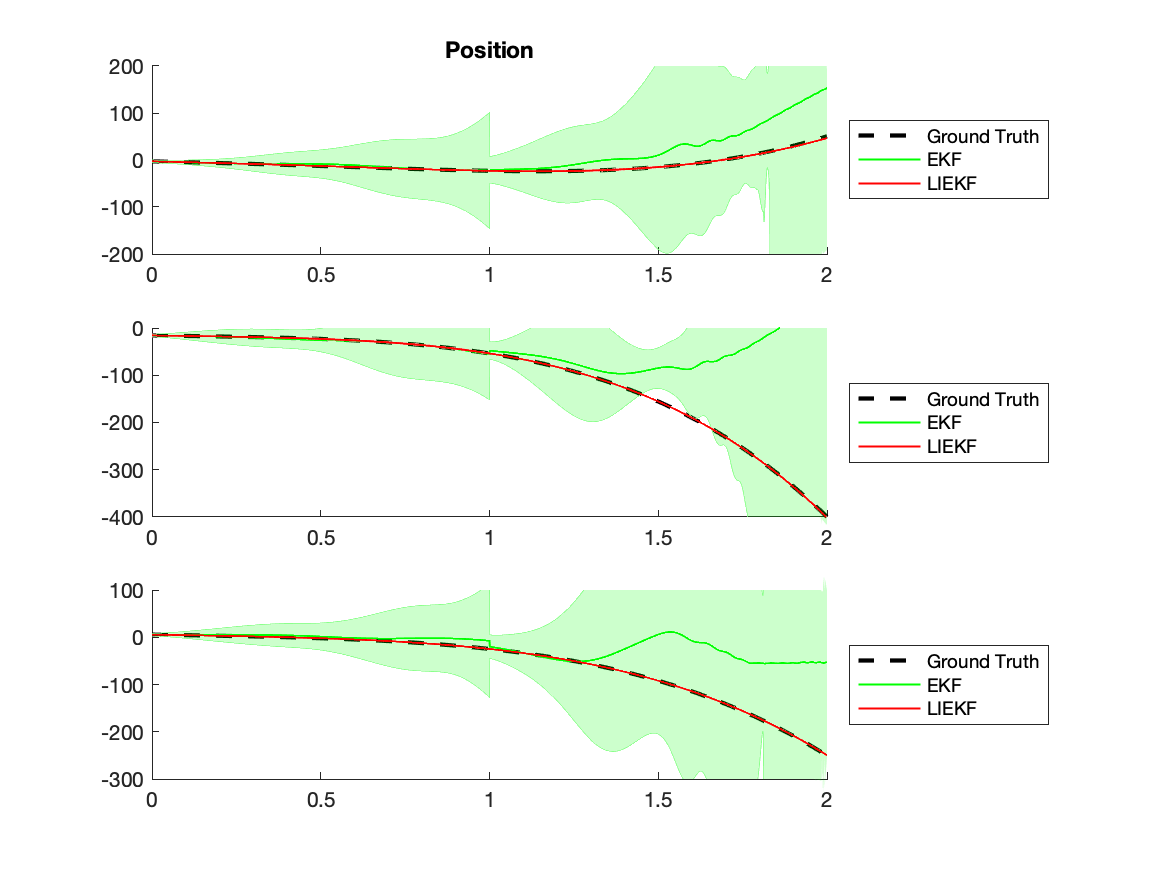
\includegraphics[width=0.45\textwidth]{sections/figures/fake_data_position_nonoise.png}
    \caption{(Simulated data, measurements without noise) EKF (solid green) and LIEKF (solid red) closely follow and converge to the ground truth (dashed black) from perturbed initial conditions. The covariance of each filter is shown as the shaded zone}
    \label{fig:fake_data_pos}
\end{figure}

\begin{figure}
    \centering
    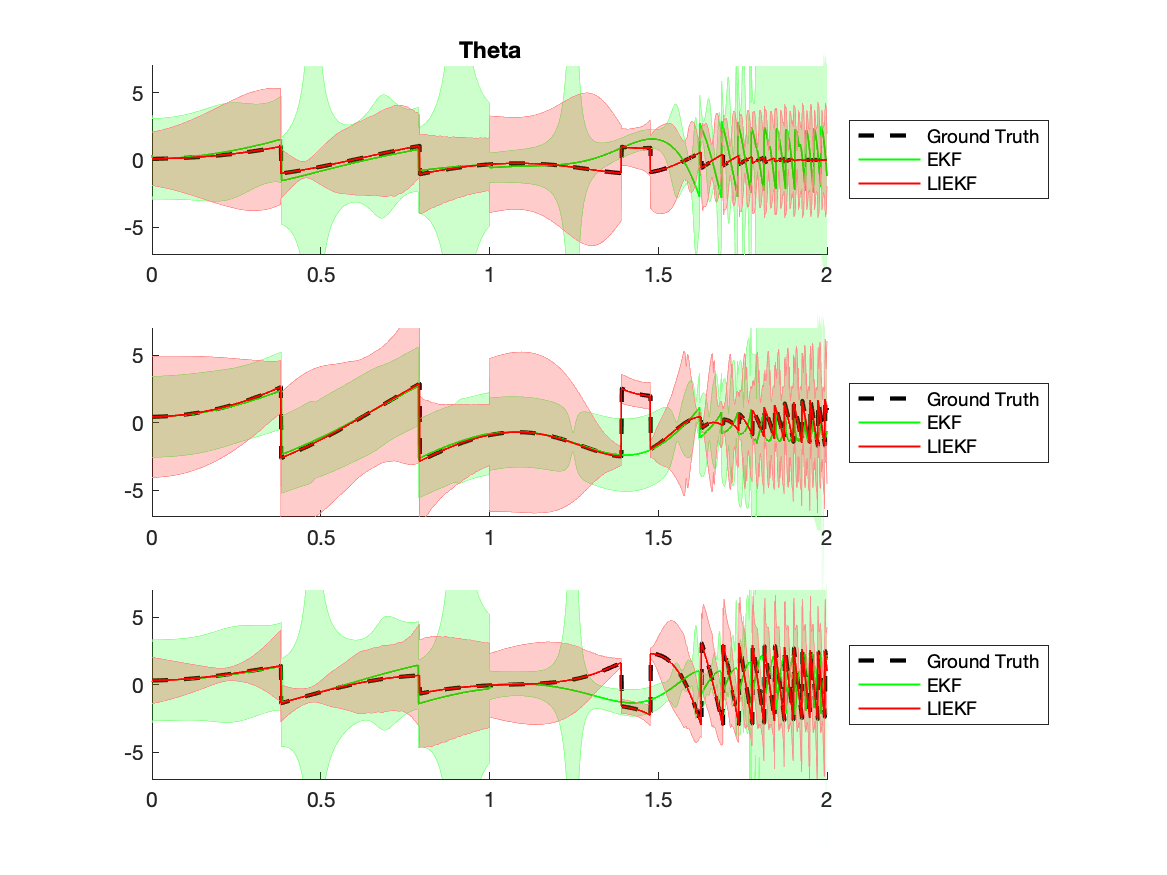
\includegraphics[width=0.45\textwidth]{sections/figures/fake_data_theta_nonoise.png}
    \caption{(Simulated data, measurements without noise) EKF (solid green) and LIEKF (solid red) closely follow and converge to the rotational state of the body. Quantity plotted is $\theta = \mathrm{Log}(R)$, where $R$ is the rotation of the body. The covariance of each filter is shown as the shaded zone}
    \label{fig:fake_data_ang}
\end{figure}

The plots in Figs.~(\ref{fig:fake_data_pos}, \ref{fig:fake_data_ang}) show a simulated run on the filter with no noise, but with position initial conditions perturbed from the ground truth.  The polynomial functions used for the position and angle are listed in Appendix (\ref{sec:fake_data}).  The plots show that the filter converges in both the position and the orientation, and continues to follow the ground truth after converging. The variance of estimation from LI-EKF is bounded well along the trajectory, demonstrating the benefits of autonomous error dynamics.

\begin{figure}
    \centering
    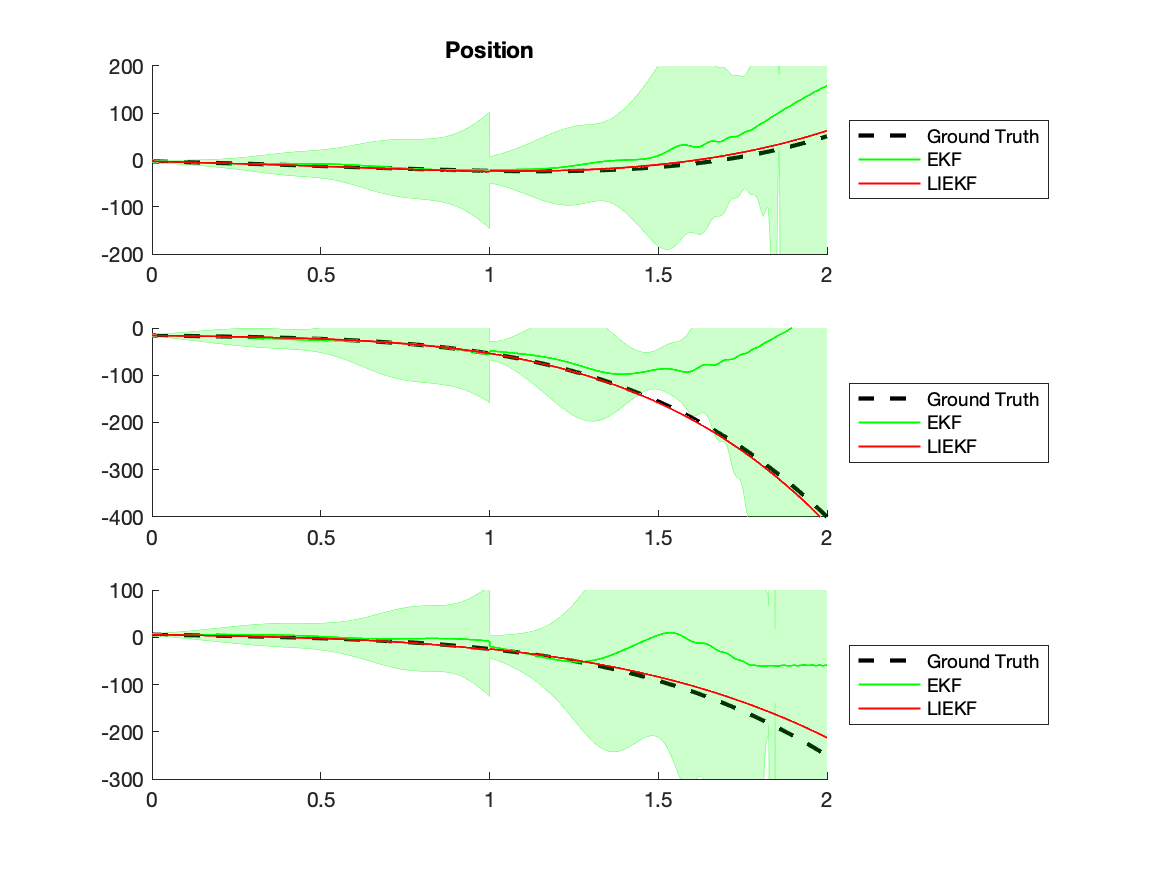
\includegraphics[width=0.45\textwidth]{sections/figures/fake_data_position_noise.png}
    \caption{(Simulated data, measurements with noise) EKF (solid green) and LIEKF (solid red) closely follows ground truth position despite noisy accelerometer reading. The covariance of each filter is shown as the shaded zone}
    \label{fig:fake_data_pos_noise}
\end{figure}

\begin{figure}
    \centering
    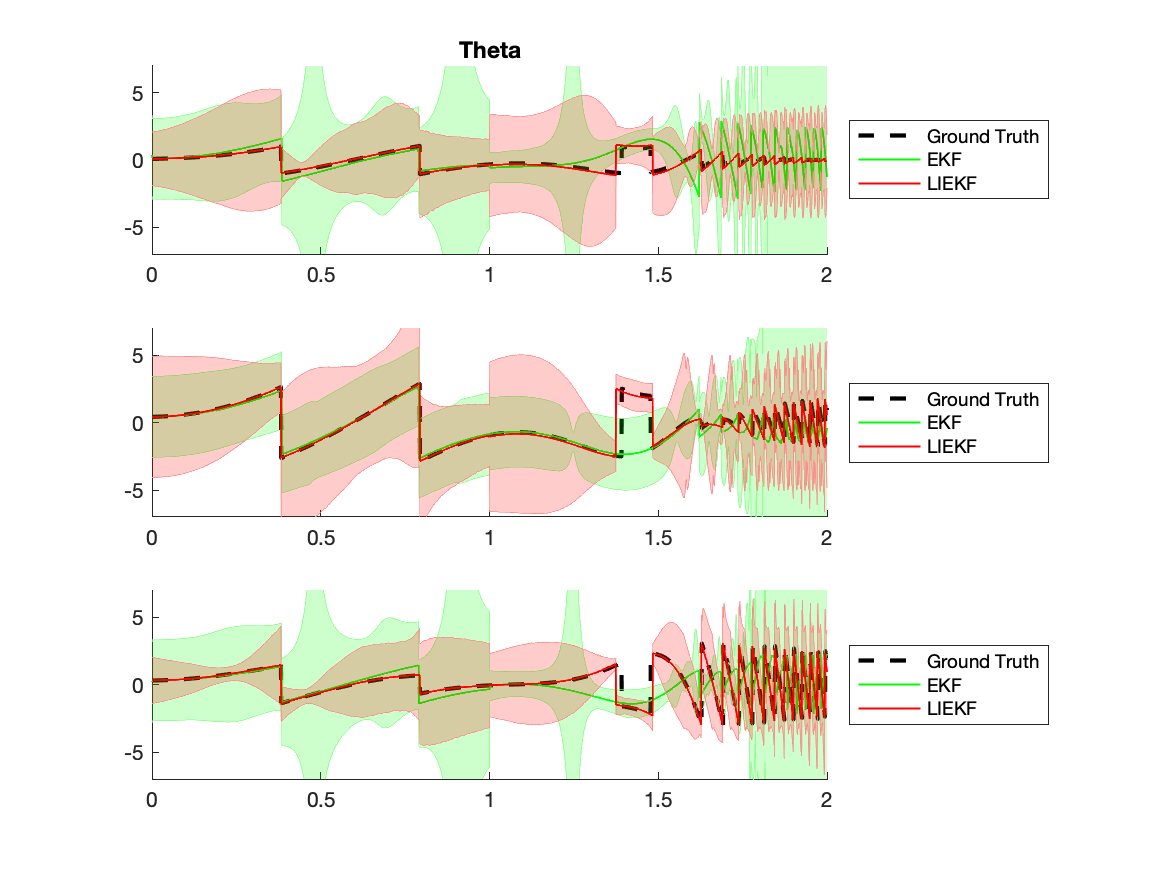
\includegraphics[width=0.45\textwidth]{sections/figures/fake_data_theta_noise.png}
    \caption{(Simulated data, measurements with noise) EKF (solid green) and LIEKF (solid red) closely follows ground truth rotation despite noisy acclerometer readings. Quantity plotted is $\theta = \mathrm{Log}(R)$, where $R$ is the rotation of the body. The covariance of each filter is shown as the shaded zone}
    \label{fig:fake_data_ang_noise}
\end{figure}

The plots in Figs.~(\ref{fig:fake_data_pos_noise},\ref{fig:fake_data_ang_noise}) show another simulated run but with some large noise added to the measurements.  In this test, we add normally disturbed, zero mean random noise with a standard deviation of 6$g$'s (58.86 m/s$^2$) to the accelerometer measurements.  Additionally we added similarly distributed noise with a standard deviation of 1 rad (57 deg) to the gyro measurements.  Initial conditions were set the ground truth and the filter was run with an update frequency of 10 Hz.  Despite the noisy conditions and the slow update rate, the filter tracked closely in position and orientation. However, there is visible disparity between the LI-EKF estimation and ground truth for velocity, especially along z-axis.  The orientation also shows less accuracy, and there is a small but noticeable steady state error in the estimation.  On another hand, the variance of the estimation is still bounded well and is not influenced much by the addition of noise.



%%%%%%%%%%%%%%%%%%%%%%%%%%%%%%%%%%%%%%%%
\subsection{Tests on Zurich Urban}
We selected the Zurich Urban data set \cite{majdik2017zurich} to test our Left-invariant EKF implementation. The data set includes GPS, accelerometer, and gyroscope measurements for a quad-rotor traversing the streets of Zurich. Additionally, the data set includes "ground-truth" data obtained using image processing. In our tests we use this estimate as our ground-truth. Using the accelerometer and gyroscope readings as our prediction step and the GPS measurements to update our prediction. The accelerometer and gyroscope update at roughly the same time step and so we assume these happen synchronously. The IMU and gyro update roughly 10 times per second. However, the GPS updates asynchronously, updating roughly once per second. To handles this, our filter runs a prediction step when it receives new IMU/gyro data and runs the correction step whenever GPS readings are received. Figures \ref{fig:Zurich_3D} and \ref{fig:Zurich_XYZ} show the results of applying our filter to the data set.

\begin{figure}
    \centering
    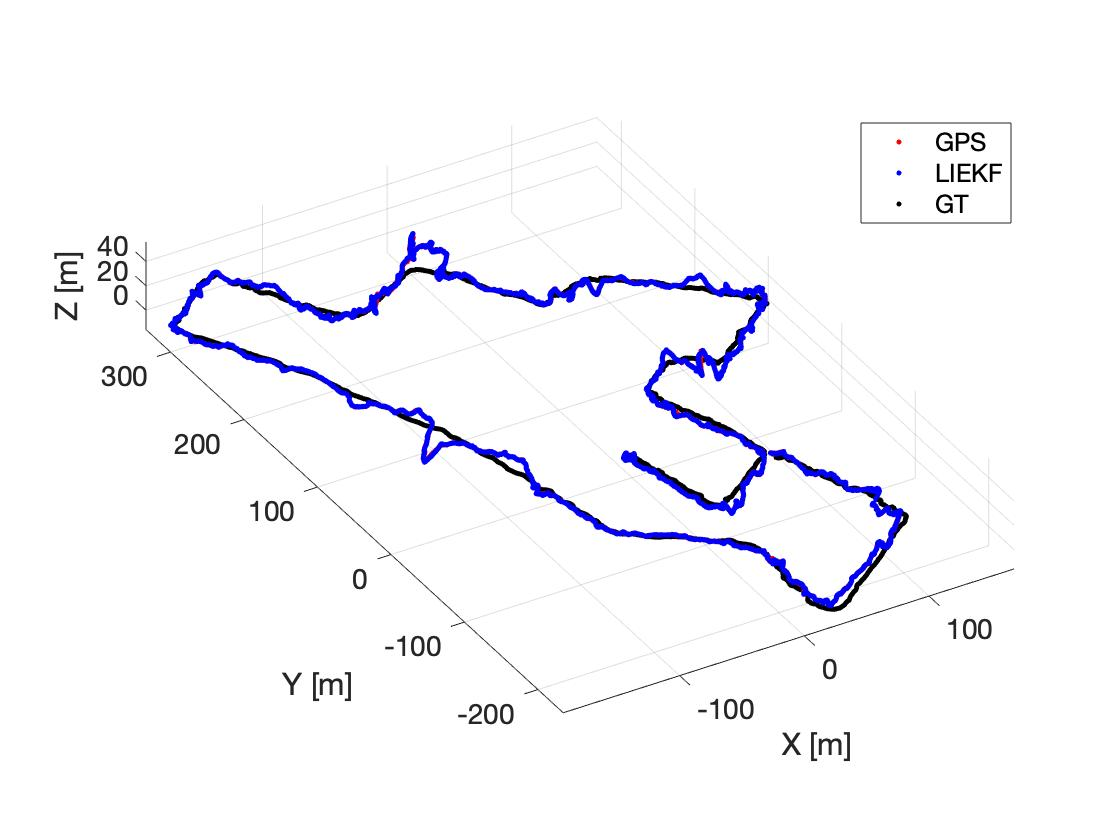
\includegraphics[width=0.45\textwidth]{sections/figures/Zurich_3D.jpg}
    \caption{The filter's state estimation on the Zurich Urban data set (blue) vs the ground truth (black). The filter follows the XY position very well, but the Z position is very noisy. The GPS readings (red) are also plotted, but are difficult to see as the estimate overlaps it in most places.}
    \label{fig:Zurich_3D}
\end{figure}

\begin{figure*}[h]
    \centering
    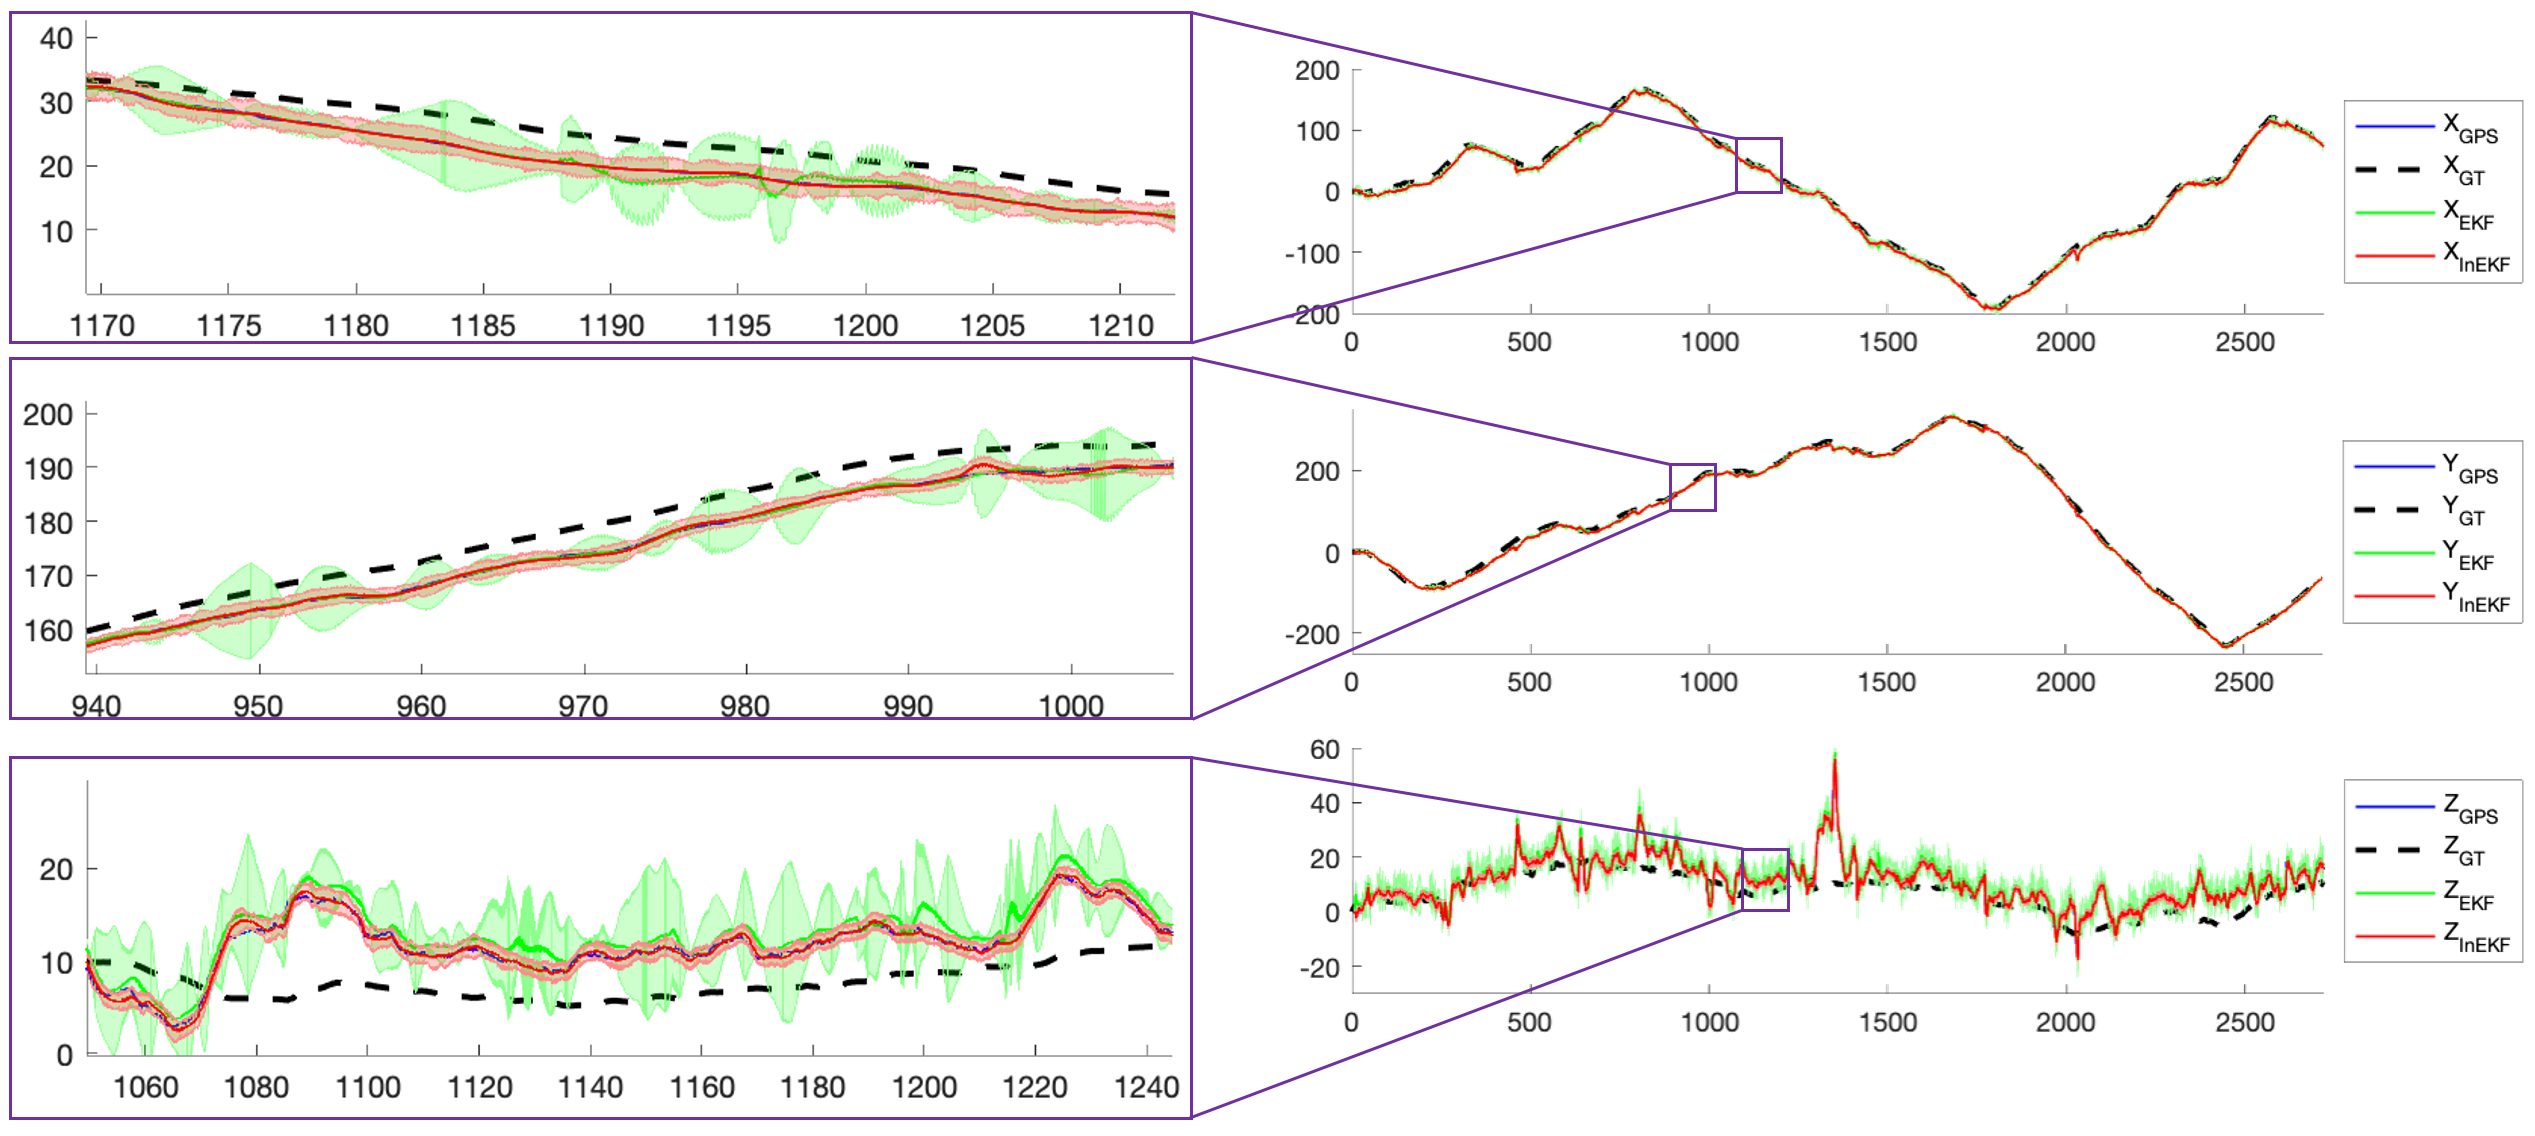
\includegraphics[width=.8\textwidth]{sections/figures/zurich_pos_std.png}
    \caption{The $x$ (top), $y$ (middle), and $z$ (bottom) positions and standard deviation of the drone over time. 
    The dashed black line is the ground truth position, and the blue line (covered by green and red) is the GPS position. The red line is the LI-EKF position and the green line is the EKF position. The shaded region is $3\sigma$ covariance. Although both trajectory follow the GPS trajectory closely, we can see that in the zoomed in version, the variance for LI-EKF is lower than the standard deviation for the EKF. This means that there is less error in the LI-EKF position}.
    \label{fig:Zurich_XYZ}
\end{figure*}

From the plots \ref{fig:Zurich_3D} and \ref{fig:Zurich_XYZ} we can see that the filter tracks the state well. However, the estimte is highly dependent upon the GPS measurements. In fact, in this case we fail to perform significantly better than just using pure GPS data. We can see in figure \ref{fig:Zurich_error} that there is some error present, but that it is nearly identical at all points to the GPS error. Even though we use a bias correction on the IMU and gyro, we fail to gain any information from their inclusion. 

The reason underneath that lies in the the quality of the measurements rather than the quality of our filter, since we have tested our filter on simulated data. Therefore, we could potentially improve the estimation results by including additional measurements such as incorporating magnetometer readings or using the gravity vector to correct the heading. Alternatively, we could add a bias correction in the measurement step which could help correct the noisy GPS data.

\begin{figure}
    \centering
    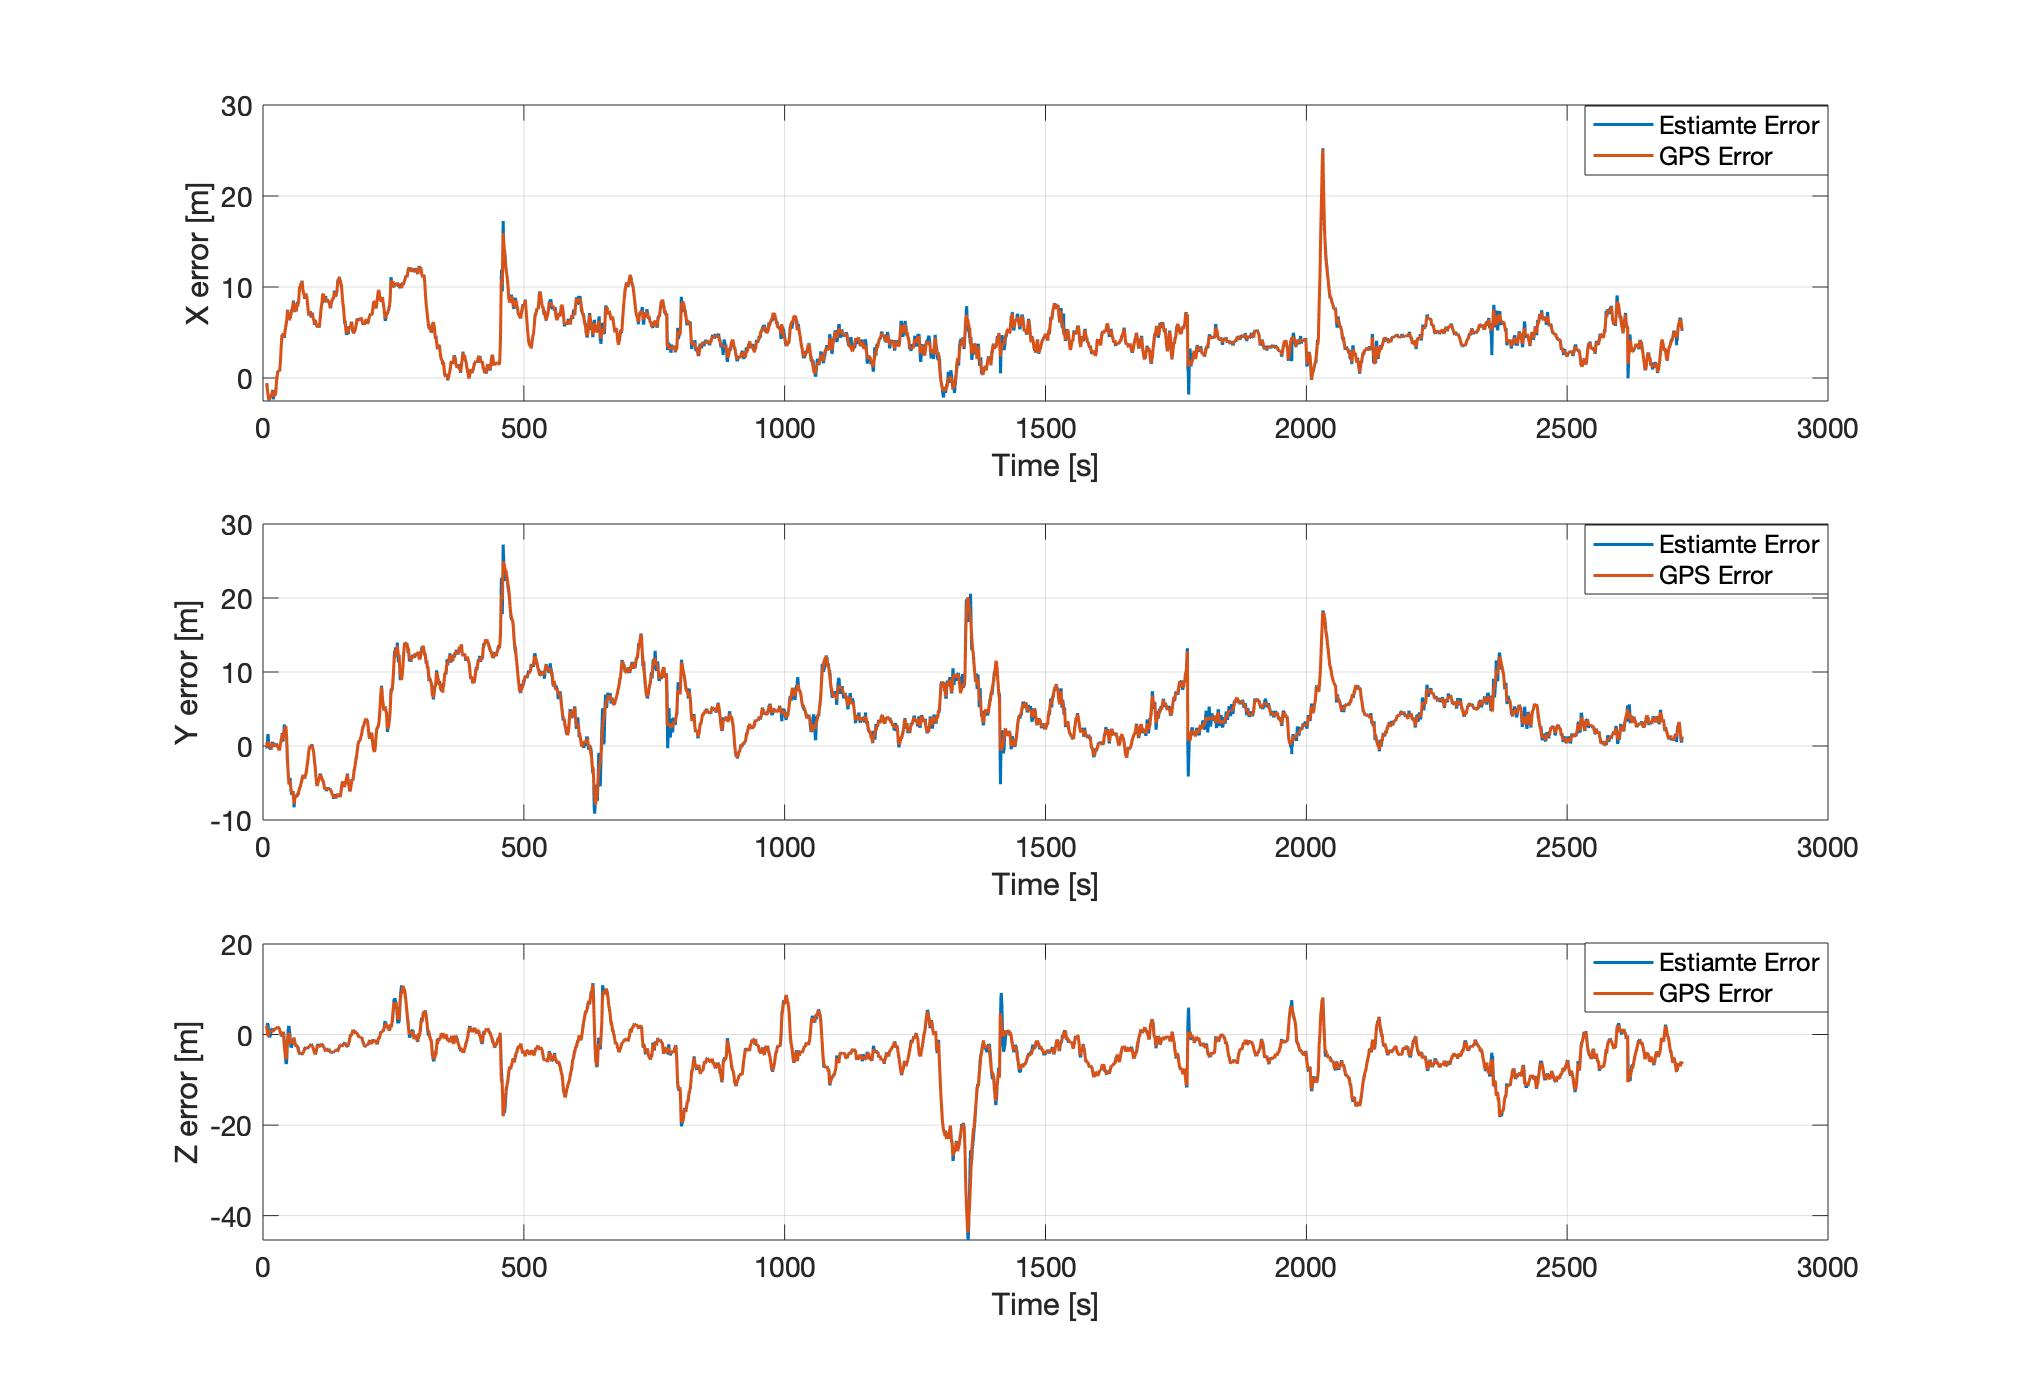
\includegraphics[width=0.45\textwidth]{sections/figures/Zurich_error.jpg}
    \caption{The X (top), Y (middle), and Z (bottom) error of the drone position over time. The LI-EKF filter error is in blue and the GPS error is in orange dashed lines. In most places these lines overlap.}
    \label{fig:Zurich_error}
\end{figure}

%%%%%%%%%%%%%%%%%%%%%%%%%%%%%%%%%%%%%%%%

\subsection{Comparison to Traditional EKF}
 As a baseline for comparison, we have developed traditional EKF algorithm in Matlab. The estimated states of the vehicle are position $\mathbf{p}(t)$, velocity $\mathbf{v}(t)$ and orientation in Euler angles $\mathbf{\phi}(t)$.

It could be observed from Figure \ref{fig:fake_data_pos} to Figure \ref{fig:fake_data_ang_noise}, with or without noise in the measurement, LI-EKF would be able to track both the position and orientation of the body accurately. In comparison, EKF magnifies local oscillation for orientation tracking, and fails to follow the ground truth position at the end when the gradient becomes steep and the nonlinearity is accumulated more, since the approximation of linearization is breached. However, the variance of LI-EKF is bounded along the trajectory because of the autonomous error dynamic of Lie algebra; however, that of EKF would grow unbounded after a short while, which also demonstrate the failing in its tracking. The inclusion of noise seems to have a small but non-critical impact on the performance of both filters, with slightly increased values of error in position and orientation tracking.

For the Zurich Urban Dataset, the advantage of LI-EKF is not obvious through visual inspection. For both of the filers, the estimation results closely follow GPS data along the trajectory, indicating the prediction from IMU is not included in the estimation process. In Figure \ref{fig:Zurich_XYZ}, it could be observed that though the estimation of the position for the two filters overlapped, the variance for LI-EKF is better bounded compared with EKF, suggesting a more reliable estimation statistically.